\chapter{Convertisseur Buck}

Le TP fait suite au TD sur le convertisseur Buck dont l'énoncé est rappelé ci-dessous.
L'objectif est d'utiliser le logiciel LTSpice afin de simuler le circuit et d'en comprendre le fonctionnement.
LTSpice est un logiciel fourni par Analog Device, basé sur de la simulation Spice. La documentation du logiciel est disponible sur le site d'Analog Device: \href{https://www.analog.com/en/resources/design-tools-and-calculators/ltspice-simulator/ltspice-recommended-reading-list.html}{Analog Device Website}

On souhaite alimenter un microprocesseur STM32H4 à l'aide d'une batterie. Le cahier des charges est le suivant :

\begin{itemize}
\item Batterie LiPo 2S $V_{in} = 7.4\ V$
\item Tension d'alimentation du microprocesseur : $V_{out}=3.3\ V$
\item Ondulation de tension max en entrée du microprocesseur : $\Delta V_S = 50\ mV$
\item Courant nominal de sortie : $I_S = 200\ mA$
\item Ondulation de courant : 30\%
\end{itemize}

Pour cela, on souhaite utiliser le composant suivant : \textbf{LT1959} dont un extrait de la documentation 
est en annexe.
On supposera dans cet exercice que les \underline{\textbf{composants sont}} 
\underline{\textbf{parfaits}}, et que le Buck fonctionne en régime de \underline{\textbf{conduction continue}}.

\section{Préparation}

\begin{enumerate}
\item Tracer le circuit permettant d'utiliser ce composant en fonctionnement Buck
\item Rappeler les valeurs de (aucun calcul n'est demandé) :
\begin{itemize}
    \item la fréquence de découpage du hacheur
    \item les valeurs de $L_1$, $C_1$ du filtrage de sortie du hacheur permettant de respecter le cahier des charges
    \item les résistances $R_1$ et $R_2$ de feedback permettant d'avoir une tension de sortie de $3.3\ V$
    \item la valeur de la résistance $R_m$ modélisant le microcontrôleur absorbant un courant nominal
    \item les valeurs de $R$ et $C$ pour l'asservissement de la tension de sortie limitant le rapport cyclique au démarrage à $\dfrac{\alpha_n}{2}$ 
    et une constante de temps du correcteur 10 fois supérieure à la constante de temps du système non corrigé
\end{itemize}
\end{enumerate}

\newpage
\section{Simulation du circuit}

Voici un bref résumé de l'interface LTSpice. Pour plus d'information, vous pouvez vous référer à la page d'Analog Device:
\href{https://www.analog.com/en/resources/design-tools-and-calculators/ltspice-simulator/ltspice-recommended-reading-list.html}{Analog Device Website}

\begin{figure}[h]
    \centering
    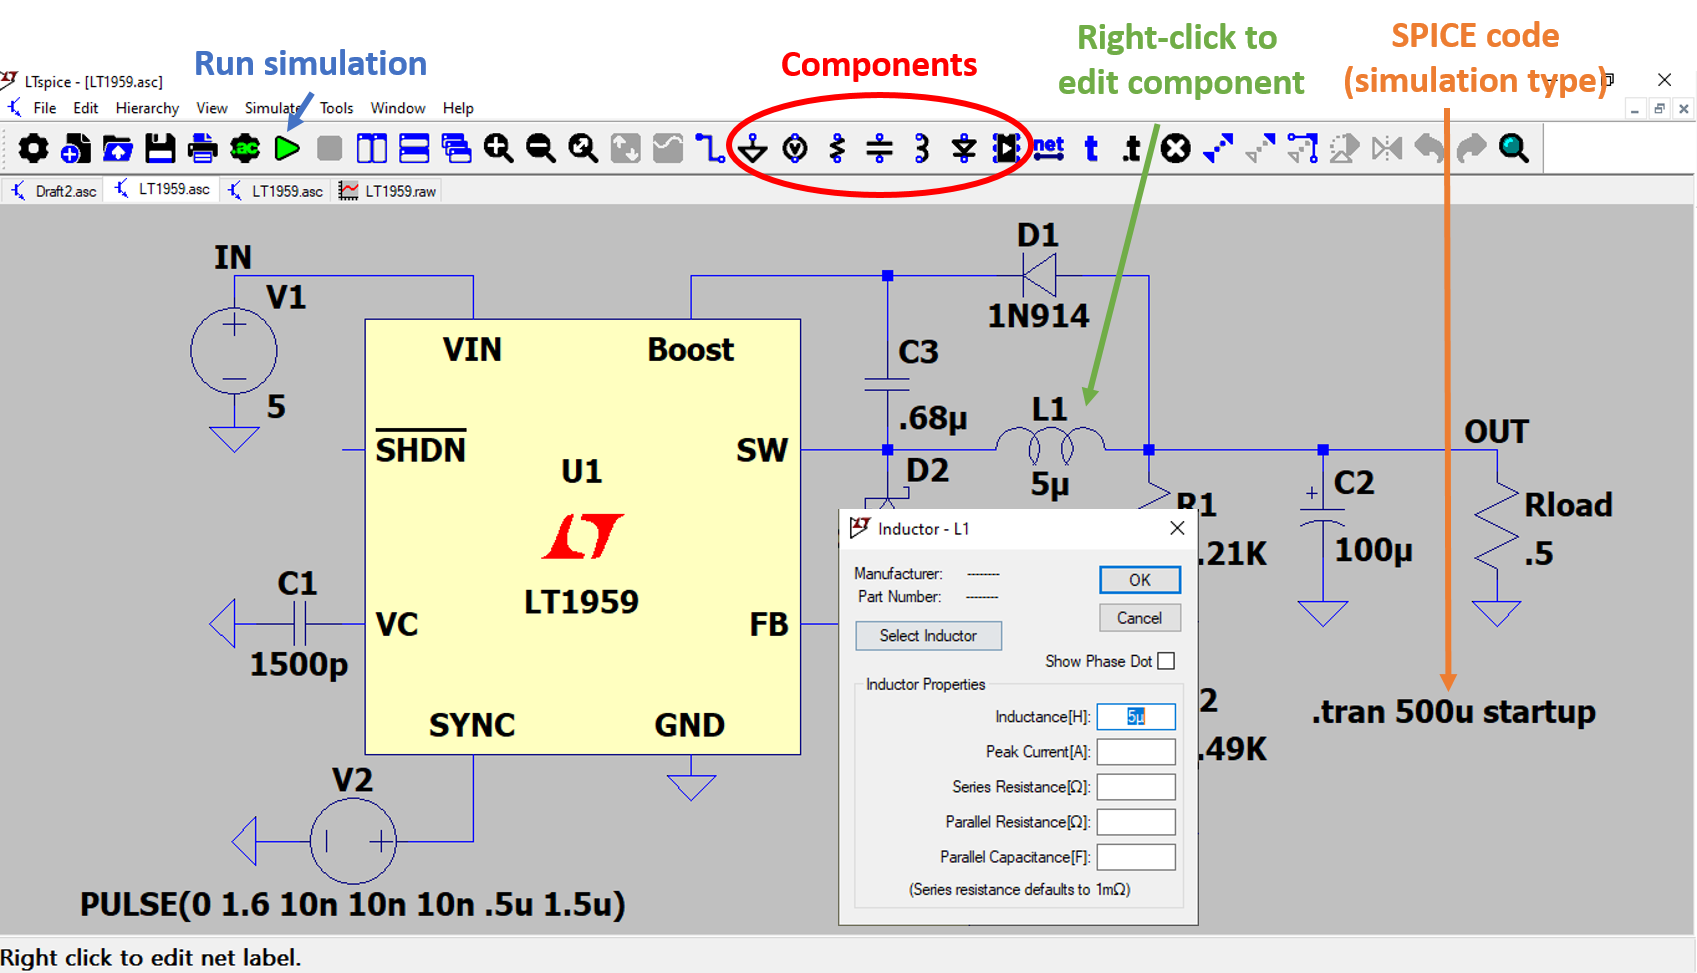
\includegraphics[width=\linewidth]{TP_Buck/fig/LTSpice.png}
\end{figure}

\begin{itemize}
\item Créer un nouveau \textit{Schematic} et placer le \textbf{LT1959}.
\item Créer le circuit de la datasheet en faisant un clic droit sur le composant $\Rightarrow$ "\textit{Open Example Circuit}"
\item Modifier le circuit pour qu'il corresponde à la datasheet. La broche "\textit{SYNC}" ne sera pas utilisée.
\item Modifier les valeurs des composants afin qu'ils correspondent au cahier des charges.
\item Réaliser une simulation temporelle. Pour cela, aller dans "\textit{Simulate}" $\Rightarrow$ "\textit{Configure Analysis}" 
$\Rightarrow$ "\textit{Transcient}" et réaliser une simulation sur 3 ms.
\end{itemize}

\begin{enumerate}
\item Vérifier la valeur de la fréquence de découpage du convertisseur
\item Vérifier que le cahier des charges est respecté : tension de sortie, ondulation de courant, ondulation de tension
\item Le convertisseur fonctionne-t-il en régime de conduction continu ou discontinu ?
\end{enumerate}


\section{Influence des composants}

\begin{enumerate}
    \item Mesurer la valeur de l'ondulation de courant dans $L_1$ et de l'ondulation de tension de sortie pour différentes valeurs de $L_1$. Commenter.
    \item Mesurer la valeur de l'ondulation de tension de sortie pour différentes valeurs de $C_1$. Commenter.
    \item Déterminer la valeur de $L_1$ pour être en régime de conduction critique. Vérifier par la simulation.
\end{enumerate}

\section{Rapidité et stabilité du système}

\begin{enumerate}
    \item Modifier la valeur de $C$ et mesurer le temps de réponse à 5\%. Commenter.
    \item En modifiant la valeur de $R$ déterminer la valeur maximale de la résistance à partir de laquelle le système devient instable.
    \item Ajouter un générateur de courant en parallèle de la résistance $R_s$ afin de générer un pulse de courant (une fois le système en régime permanent). 
    Ce pulse peut modéliser un appel de courant brusque du système alimenté par le Buck. Déterminer la nouvelle valeur de $R$ à partir de laquelle le système devient instable lors d'une perturbation.
\end{enumerate}